\section{Spectral clustering}
L'idée centrale des techniques de clustering spectral est qu'un graphe est représentable par une matrice à partir de laquelle on peut utiliser les techniques d'analyse de l'algèbre linéaire.

Un graphe $G$ est la donnée d'un couple $(V, E)$ tel que $V$ est une ensemble de nœuds et $E$ et un ensemble d'arêtes (i.e un couple $(i,j)$ où $i,j \in V$).
A partir de cette définition on peut représenter le graphe par une matrice dont les éléments correspondent à certaines données de $G$.
Il existe tout un ensemble de matrices représentant le graphe:
\begin{itemize}
  	\item[-]  Adjencency Matrix $= A$;
  	\item[-]  Laplacian Matrix $= L$;
  	\item[-]  Modularity Matrix $= M$;
  	\item[-]  Bethe Hessian Matrix $= H$;
  	\item[-]  "$\alpha$-normalized” Adjacency Matrix $= D$.\\
\end{itemize}
Par exemple, la matrice d'adjacence d'un graphe, notée $A$, est définie telle que $\forall i,j \in V, \; A_{ij} = \mathbbm{1}_{(i,j) \in E}$.
Une colonne $i$ représente le nœud $i$ dont chaque composante, $j$, est égale à $1$ si il existe une arête entre $i$ et $j$ et $0$ sinon.\\

Ci-dessous un graphe qui permettant d'avoir une vue d'ensemble sur l'avancement des méthodes de spectrales de détection de communautés.
Cette liste n'est pas exhaustive.
\begin{figure}[H]
\centering
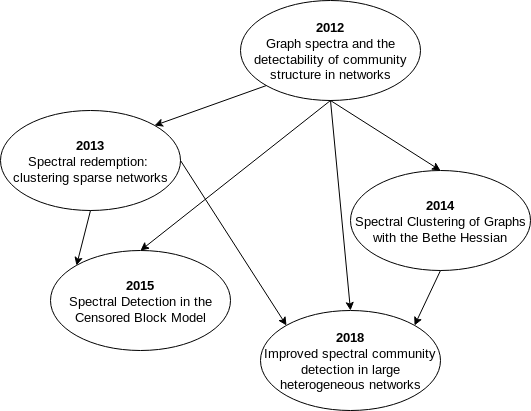
\includegraphics[scale=0.5]{static/graph_research.png}
\caption{graphe des différentes méthodes de ``graph spectral clustering''}
\end{figure}

\subsection{Algorithme de clustering spectral de graphe}
 \label{par:algo spectral clustering}
La procédure pour associer une communauté aux nœuds de $G$ via une méthode spectrale est la suivante: 
\begin{itemize}
	\item[1-] Calcul des vecteurs propres, $v_i$, d'une matrice représentant le Graphe $G$ ;
	\item[2-] Sélection des $l$ vecteurs propres portant l'information de la structure de communauté ; 
	\item[3-] Construction de la matrice $W = [v_1, \cdots, v_l] \in \mathbb{R}^{n\times l}$ ; 
	\item[4-] Projection des vecteur lignes $r_j$ de $W$ sur l'espace de dimension $l$, où chaque $r_j$ correspond  au nœud $j$ ; 
	\item[5-] Catégorisation des vecteurs $r_j $ dans une communauté via des algorithmes de clustering: \textit{K-Means}, \textit{Expetation-Maximization}, \textit{Support vector machine }, etc.\\
\end{itemize}

\par{\underline{Étape 1:}}
La matrice $A$ est carrée, par conséquent elle peut être interprétée comme la représentation d'un endomorphisme dans un espace X de dimension $n$ (nombre de nœuds dans $G$).
Soit la base canonique $(e_i)_{i=1:n}$, chaque $e_i$ correspond au nœud $i$.
Les vecteurs propres de $A$ sont donc des combinaisons linéaires des nœuds de $G$.
Les nœuds concernés ont donc une certaine dépendance.
\par{\underline{Étape 2:}}
Les entrées de la Matrice $A$ sont modélisées par des variables aléatoires vérifiant certaines hypothèses (e.g centrées, moments finis, indépendantes ...).
La théorie des matrices aléatoires nous dit qu’asymptotiquement la mesure spectrale de A converge vers une loi déterministe $\mu$ (loi qui dépend de la matrice étudiée).
Les valeurs propres de $A$ distribuées selon $\mu$ peuvent être interprétées comme du bruit lié aux fluctuations aléatoires des simulations.
Elles nous renseigne en rien sur la structure non aléatoire des entrées de $A$ .\\
Cependant, lorsque le graphe admet une structure de communauté, les entrées ne sont plus tout à fait indépendantes.
Dans ce cas de figure, la théorie prévoit que des valeurs propres sortent du support de la mesure spectrale $\mu$.
Ce sont ces valeurs propres qui contiennent l'information de la structure de communauté de $G$.\\
Autrement dit, si la structure de communauté de $G$ n'est pas assez ``explicite'', les valeurs propres censées porter l'information des communautés ne sortiront pas du support de la mesure spectrale théorique, et donc, seront interprétées comme du simple bruit.
Dans cette situation, la méthode spectrale est incapable de déceler la structure de communauté de $G$.
\par{\underline{Étape 4:}}
Les vecteurs colonnes de W correspondent à des combinaisons linéaires de nœuds.
De par la construction de A, les entrées $i$ de ces vecteurs colonnes sont la somme des arêtes entre les nœuds sous-jacent et le nœud $i$.
Les vecteurs propres que l'on a gardés sont ceux qui portent l'information des communautés.
Donc chaque vecteur ligne représente un nœud du graphe et l'espace dans lequel il se meut constitue l'information de la structure de communauté.\\

Les algorithmes de détection de communauté spectraux à partir des opérateurs linéaires tels que la matrice ``non-backtracking'' et la matrice ``Bethe Hessian'' sont similaires et sont décrits dans l'article \cite[Spectral detection in the censored block model]{Spectral_Detection_in_the_Censored_Block_Model}.

\subsection{Non-backtracking matrix}
La matrice Non-backtracking est un opérateur linéaire sur lequel se base de nombreuses récentes recherches.
Elle se construit de la manière suivante   
\subsubsection{Localization and Centrality in Networks }
\subsubsection{Spectral Redemption: Clustering Sparse Networks}
\subsubsection{Percolation on Sparse Networks}
